% Include stability analysis

\section{Stability of Lagrange Points}

To assess the stability of a spacecraft's trajectory near the Lagrange points, we need to consider the equations of motion linearized near these points of equilibrium in the CR3BP.

\vspace{\baselineskip}

For a nonlinear time-invariant system $\dot{x} = f(x)$ where $x, f \in \mathbb{R}^n$, and $\bar{x}$ represents an equilibrium point, i.e. $f(\bar{x})=0$, we investigate the localized behavior by considering small deviations
$\delta x$ from the equilibrium. Consider a point $x$ near $\bar{x}$, i.e. $x = \bar{x} + \delta x$. Expanding the system about $\bar{x}$ through a Taylor series and disregarding higher-order terms yields:
\begin{equation}
    \delta \dot{x} = J(\bar{x}) \, \delta x
\end{equation}

where $J(\bar{x}) = \ddfrac{\textrm{D}f}{\textrm{D}x} (\bar{x})$ is the Jacobian matrix of $f$ evaluated at the equilibrium $\bar{x}$. This differential equation represents a linear approximation governing the evolution of deviations $\delta x$ in a small neighborhood. 

\vspace{\baselineskip}

Let $L$ denote any of the Lagrange points $L_1$ to $L_5$. Let's find the linearized CR3BP equations around the Lagrange point $L$ with the generalized coordinates $\bar{x} = (x_L,y_L,\dot{x}_L,\dot{y}_L) = (x_L,y_L,0,0)$:

\subsection{Linearization of Equations of Motion}

Recall the set of ODEs:

\begin{equation*}
    \begin{pmatrix}
        \dot{x}   \\
        \dot{y}   \\
        \dot{v}_x \\
        \dot{v}_y
    \end{pmatrix} =
    \begin{pmatrix}
        v_x                                                                                                        \\[0.2cm]
        v_y                                                                                                        \\[0.2cm]
        2v_y + x - \ddfrac{(1-\mu) \left(x+\mu\right)}{r_1^3} - \ddfrac{\mu \left(x-1+\mu\right)}{r_2^3} - f_d v_x \\[0.2cm]
        -2v_x + y - \ddfrac{1-\mu y}{r_1^3} - \ddfrac{\mu y}{r_2^3} - f_d v_y
    \end{pmatrix}
    = f(x,y,v_x,v_y)
\end{equation*}

The associated Jacobian for these dynamics is a 4 $\times$ 4 matrix:

\begin{equation*}
    J(\bf{X}) =
    \begin{pmatrix}
        \pderiv{f_1}{x} &  & \pderiv{f_1}{y} &  & \pderiv{f_1}{v_x} &  & \pderiv{f_1}{v_y} \\[0.4cm]
        \pderiv{f_2}{x} &  & \pderiv{f_2}{y} &  & \pderiv{f_2}{v_x} &  & \pderiv{f_2}{v_y} \\[0.4cm]
        \pderiv{f_3}{x} &  & \pderiv{f_3}{y} &  & \pderiv{f_3}{v_x} &  & \pderiv{f_3}{v_y} \\[0.4cm]
        \pderiv{f_4}{x} &  & \pderiv{f_4}{y} &  & \pderiv{f_4}{v_x} &  & \pderiv{f_4}{v_y}
    \end{pmatrix}
\end{equation*}

Under the assumption $f_d$ = 0, this simplifies to:

\begin{equation}
    J(\bf{X}) =
    \begin{pmatrix}
        0               &  & 0               &  & 1  &  & 0 \\[0.4cm]
        0               &  & 0               &  & 0  &  & 1 \\[0.4cm]
        \pderiv{f_3}{x} &  & \pderiv{f_3}{y} &  & 0  &  & 2 \\[0.4cm]
        \pderiv{f_4}{x} &  & \pderiv{f_4}{y} &  & -2 &  & 0
    \end{pmatrix} %\right|_{\substack{x = x_L \\ y = y_L}}
    \label{eq:Jacobian}
\end{equation}

\pagebreak

where
\begin{align*}
    \pderiv{f_3}{x}                   & = 1  - \frac{(1-\mu)}{{r_1 }^{3} } - \frac{\mu }{{r_2 }^{3} } + \frac{3\,{\left(1- \mu\right)}\,{\left(x + \mu\right)^2}}{{r_1 }^{5} } + \frac{3\,\mu \,{\left(x - 1 + \mu\right)^2}}{{r_2 }^{5} }
    \\[0.4cm]
    \pderiv{f_3}{y} = \pderiv{f_4}{x} & = \frac{3\,{\left(1-\mu\right)}\,{\left(\mu +x \right)}\,y}{r_1^{5} } + \frac{3\,\mu\,{\left(x - 1 + \mu\right)}\,y}{r_2^{5} }
    \\[0.4cm]
    \pderiv{f_4}{y}                   & = 1 - \frac{1 - \mu}{{r_1 }^{3} } - \frac{\mu }{{r_2}^{3} } + \frac{3 \,{\left(1 - \mu\right)\,{y }^2}}{{r_1 }^{5} }+\frac{3\,\mu \,{y }^2 }{{r_2 }^{5} }
\end{align*}

\subsection{Stability of \texorpdfstring{$L_4$ and $L_5$}{L4 and L5}}
The points $L_4$ and $L_5$ are recognized as stable equilibria for specific values of $\mu$. To demonstrate this, let's consider $L_4$, where $\bar{x} = (x_{L4}, y_{L4}, 0, 0) = (1/2 - \mu, \sqrt{3}/2, 0, 0)$. Subsituting these values into the Jacobian from \eqref{eq:Jacobian} yields:

\begin{equation*}
    J(\bar{x}) =
    \begin{pmatrix}
        0      &  & 0      &  & 1  &  & 0 \\[0.4cm]
        0      &  & 0      &  & 0  &  & 1 \\[0.4cm]
        0.75   &  & 1.2675 &  & 0  &  & 2 \\[0.4cm]
        1.2675 &  & 2.25   &  & -2 &  & 0
    \end{pmatrix}
\end{equation*}

The dynamics in the vicinity of the equilibrium point are governed by $J$. By conducting an eigen-analysis and examining the characteristic equation $\det(J-\lambda\bf{I}) = 0$, where \textbf{I} denotes the $4\times4$ identity matrix, we can assess the stability. The characteristic equation is given by:

\begin{equation*}
    \det(J-\lambda\bf{I}) =
    \left|\begin{matrix}
        -\lambda &  & 0        &  & 1        &  & 0        \\[0.4cm]
        0        &  & -\lambda &  & 0        &  & 1        \\[0.4cm]
        0.75     &  & 1.2675   &  & -\lambda &  & 2        \\[0.4cm]
        1.2675   &  & 2.25     &  & -2       &  & -\lambda
    \end{matrix}\right|
\end{equation*}

This reduces to the following polynomial:
\begin{equation}
    p(\lambda) = \lambda^4 + \lambda^2 + 0.08087 = 0
\end{equation}

The roots to $p(\lambda)$ correspond to the eigenvalues of $J(\bar{x})$:
\begin{equation*}
    \lambda = \pm 9.546i, \pm 0.2979i
\end{equation*}

Given that the real parts of $\lambda$ equal zero, implying purely imaginary eigenvalues, it indicates \fcolorbox{white}{black}{\cm neutral stability} concerning the Lagrange point. A similar result can be derived for $L_5$. In practice, however, the stability remains undetermined due to the omission of higher-order terms in the Taylor series expansion. Nevertheless, it is observed that for small deviations from these two equilibrium points, bounded oscillatory motion is generally expected within the framework of the Circular Restricted Three-Body Problem (CR3BP) in a rotating reference frame.

\pagebreak

The same analytical approach applies to Lagrange points $L_1$, $L_2$, and $L_3$. These points are widely acknowledged as unstable, as the eigenvalues of their linearized dynamics reveal at least one positive real part. Below, a figure illustrates the stability/instability of all five Lagrange points with small perturbations as initial conditions for simulating each trajectory.

\begin{figure}[h]
    \centering
    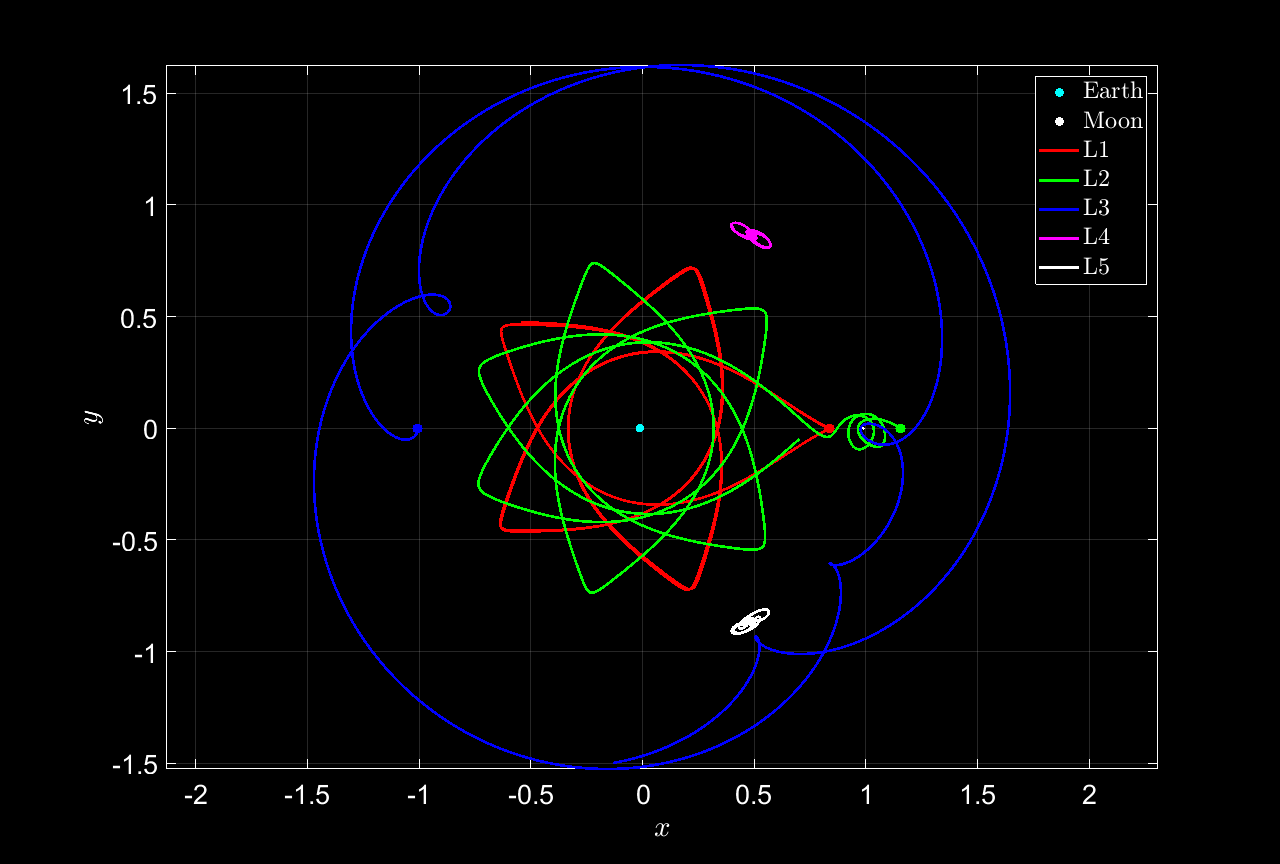
\includegraphics[width=\textwidth]{fig/lagrangeStability.png}
    \caption{Illustration of Lagrange Point Stability Considering Small Perturbations as Initial Conditions}
    \label{fig:stability}
\end{figure}

The figure above reaffirms the instability of $L_1$ to $L_3$, while indicating neutral stability for $L_4$ and $L_5$, as anticipated.